%!TeX  root  =  user_guide.tex

\chapter{Using QGIS Core Plugins}\label{sec:core_plugins}\index{plugins!core}

% when the revision of a section has been finalized, 
% comment out the following line:
%\updatedisclaimer


{\setlength{\extrarowheight}{15pt}
\small
\begin{longtable}{|p{1.2cm}|p{3.8cm}|p{10.5cm}|}
\caption{22 QGIS Core Plugins}\label{tab:core_plugins} \\
\hline
 \textbf{Icon} & \textbf{Plugin} & \textbf{Description}\\
\endfirsthead
\hline
\textbf{Icon} & \textbf{Plugin} & \textbf{Description}\\
\endhead
\hline

\includegraphics[width=0.6cm]{delimited_text}
 & Add Delimited Text Layer \index{plugins!delimited text} & Loads and displays delimited text files containing x,y coordinates\\
\hline

\includegraphics[width=0.6cm]{coordinate_capture}
 & Coordinate Capture \index{plugins!coordinate capture}& Capture mouse coordinate in different CRS\\
\hline 
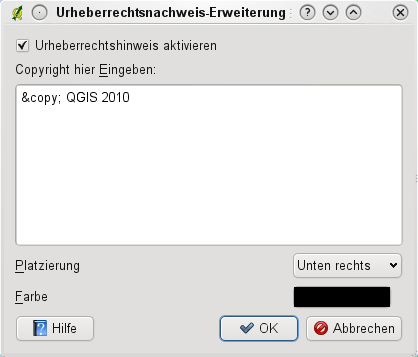
\includegraphics[width=0.6cm]{copyright_label}
 & Copyright Label \index{plugins!copyright}& Draws a copyright label with information\\
\hline

\includegraphics[width=0.6cm]{diagram_overlay}
 & Diagram Overlay \index{plugins!diagram}& Place charts (pie or bar) or proportional symbols over vector layers\\
\hline

\includegraphics[width=0.6cm]{dxf2shp_converter}
 & DXF2Shape Converter \index{plugins!DXF2Shape}& Converts from DXF to SHP file format\\
\hline
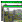
\includegraphics[width=0.6cm]{evis_icon}
 & eVis & Event Visualization Tool \\
\hline

\includegraphics[width=0.6cm, height=0.6cm]{ftoolslogo}
 & fTools \index{plugins!ftools}& A suite of analysis, geometry, geoprocessing, and research tools\\
\hline
% 
\includegraphics[width=0.6cm, height=0.6cm]{ftoolslogo}
 & GDAL Tools \index{plugins!gdaltools} & Raster tools: simplified graphical interface for most commonly used programs\\
\hline

\includegraphics[width=0.6cm]{gps_importer}
 & GPS Tools \index{plugins!gps}& Tools for loading and importing GPS data\\
\hline

\includegraphics[width=0.6cm]{grass}
 & GRASS \index{plugin!grass toolbox} & Activates the mighty GRASS Toolbox\\
\hline
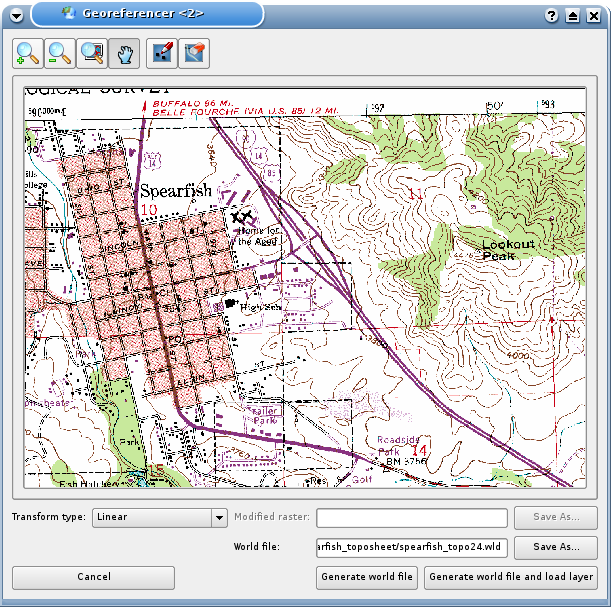
\includegraphics[width=0.6cm]{georeferencer}
 & Georeferencer GDAL \index{plugin!georeferencer} & Adding projection info to Rasterfiles using GDAL\\
\hline

\includegraphics[width=0.6cm]{interpolation}
& Interpolation plugin \index{plugins!Interpolation}& Interpolation on base of vertices of a vector layer\\
\hline

\includegraphics[width=0.6cm]{raster_terrain}
& Raster Terrain Modelling \index{plugins!Raster Terrain Modelling}& Compute slope, aspect,
ruggedness and total curvature of DEMs\\
\hline

\includegraphics[width=0.6cm]{mapserver_export}
& MapServer Export Plugin \index{plugins!MapServer Export}& Export a saved QGIS project file to a MapServer map file \\
\hline
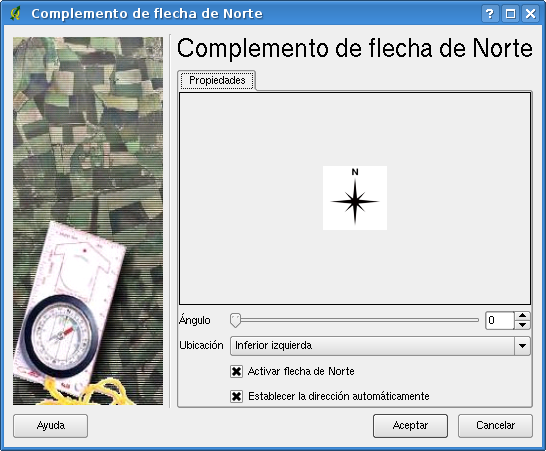
\includegraphics[width=0.6cm]{north_arrow}
& North Arrow \index{plugins!north arrow}& Displays a north arrow overlayed onto the map\\
\hline

\includegraphics[width=0.6cm]{ogr_converter}
 & OGR Layer Converter \index{plugins!OGR converter} & Translate vector
layers between OGR suported formats\\
\hline
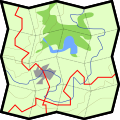
\includegraphics[width=0.6cm]{osm_icon}
 & OpenStreetMap & Visualize and edit OpenStreetMap data \\
\hline

\includegraphics[width=0.6cm]{oracle_raster}
 & Oracle Georaster \index{plugins!georaster}& Access Oracle Spatial GeoRasters\\
\hline

\includegraphics[width=0.6cm]{plugin_installer}
 & Plugin Installer \index{plugins!Plugin Installer} & Downloads and installs QGIS python plugins\\
\hline

\includegraphics[width=0.6cm]{spiticon}
 & SPIT \index{plugins!spit}& Shapefile to PostgreSQL/PostGIS Import Tool \\
\hline

\includegraphics[width=0.6cm]{quick_print}
 & Quick Print \index{plugins!quick print}& Quickly print a map with minimal
effort \\
\hline
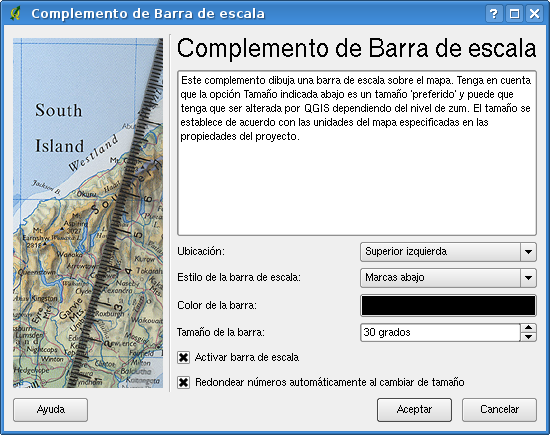
\includegraphics[width=0.6cm]{scale_bar}
 & Scalebar \index{plugins!scalebar}& Draws a scale bar\\
\hline

\includegraphics[width=0.6cm]{mIconAddWfsLayer}
 & WFS & Load and display WFS layer \\
\hline
\end{longtable}}
